\section{Composition Losses}
\label{sec:losses}

% VALUE: the expert designs lose end-to-end time in how operators are composed and issued, not in their kernels; prefill loses it between and inside operators through the CP's order, decode inside one design through its buffering and fixed placement
In this section, we characterize where the expert designs of Section~\ref{subsec:prefill} lose end-to-end time on the NPU.
In both prefill and decode, the time is lost in how the operators are composed and issued, and the remedy differs: prefill needs a different schedule of its operators, whereas decode needs a different design.

\subsection{Prefill}
\label{subsec:loss-prefill}

\begin{figure}[t]
    \centering
    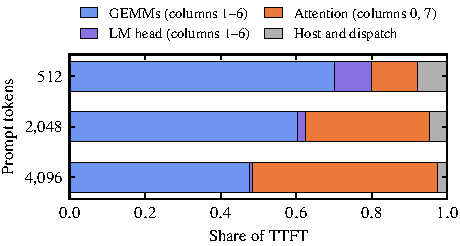
\includegraphics[width=\linewidth]{fig/busy.pdf}
    % VALUE: in the existing prefill, attention's share grows with prompt length, and each column group idles while the other computes
    \caption{Share of TTFT of the existing Llama-3.2-1B prefill by prompt length. Device-busy parts are each operator's time when dispatched alone, less the dispatch floor, summed over the prefill.}
    \label{fig:busy}
\end{figure}

% VALUE: the existing prefill issues one operator per command, so its column groups take turns; the device is busy almost all the time, but on one group at a time, and attention's growing share is time the GEMM columns sit idle
The existing prefill issues one operator per command, which amounts to about 1{,}500 commands for a 2{,}048-token prompt.
Figure~\ref{fig:busy} shows the resulting split of TTFT: device-busy time accounts for 92--97\% of it, and attention's share grows from 12\% to 49\% between 512 and 4{,}096 tokens.
Because the commands run in submission order, columns 1--6 idle while attention runs, and columns 0 and 7 idle while the GEMMs run.
The device is thus busy almost all of the time, but on only one column group at a time.
% SOURCE: commands = 16 layers x chunks x 6 + 11 LM-head commands = 1,547 at 2,048 tokens (vault lab-prefill-census (1)).
% SOURCE: amd-npu e3acc8a prefill-e2/decomp.txt via figs/make_figs.py: busy = isolated time - dispatch floor = 92/95/97% of TTFT at 512/2k/4k; of TTFT, attention 12.2/32.9/49.1%, GEMMs 70.1/60.3/47.6%, LM head 9.7/2.1/0.8%.
% SOURCE: serial execution, the isolated busy times sum to at most TTFT (vault lab-prefill-device (4)); queued commands do not overlap (Section 4).

% VALUE: the same loss occurs inside one operator: the existing attention stream starts column 7 only after waiting on column 0, which costs a third of attention's device time
The same loss occurs inside a single operator.
The existing attention stream issues column~7's inputs only after two synchronizations on column~0's key and value transfers, which complete when column~0 is about half done.
Alternating the two columns' segments, so that both columns start before the CP waits on either, reduces attention's device-busy time to $0.67\times$ that of the existing order at every chunk measured, with bit-identical outputs.
Each column's half alone takes the same time within 1\%, so the difference comes from the CP's instruction order rather than from an imbalance of work.
Since attention's share grows with the prompt, this loss grows with it.
% SOURCE: decoded from the shipped a_32_4_0_0 stream, mid-stream synchronizations at ops 70, 75 (column 0) and 92, 97 (column 7); column 7's issue (ops 81-91) follows column 0's two mid-stream synchronizations (vault lab-prefill-overlap (4)).
% SOURCE: (alternated - F) / (existing - F) = 0.666-0.668 on 7 pairs, chunks 2-14 at 2,048 tokens; column 7 alone / column 0 alone = 0.994-1.010 (amd-npu 17f7ec3 ovl4/, vault lab-prefill-overlap (5)c); 0.66-0.68 at absolute chunks 16-255 on both models (vault lab-agent-step (4)).

\subsection{Decode}
\label{subsec:loss-decode}

% VALUE: decode's per-token time grows linearly with context and attention becomes most of it; attention reads the KV cache at half the platform's read rate
The existing decode design places attention's cores on columns 3 and 4 and reads the KV cache through those columns' two shim tiles.
Its time per token grows linearly with the context length, within 0.2\% between 2{,}048 and 32{,}704 tokens, and attention's share of that time grows from 13\% at 2{,}048 tokens to 70\% at 32{,}704 tokens.
During attention, the design reads the KV cache at 51\% of the DRAM read cap measured in the same batch, and at 61\% of what two shim tiles read on their own.
% SOURCE: per-token time = 15.94 ms + 1.156 us x L, max residual 0.2% over L = 2,048-32,704 (Llama-3.2-1B, one 32k-window build, median of 3); 32 KiB per position / 1.156 us = 28.4 GB/s against a same-batch 8x2 cap of 55.2 GB/s and a 2x2 (two-shim) probe of 46.6 GB/s; attention 13/23/37/54/70% of per-token time at 2k/4k/8k/16k/32k (vault lab-decode-long-context (5)).
% SOURCE: footprint from the build's npu.air.mlir: KV readback on shims 3 and 4 (K on channel 0, V on channel 1), attention cores on columns 3 and 4 (vault lab-decode-long-context (6)).

% VALUE: the cause is the design's composition: the KV transfer alone reaches the two-shim ceiling, but compute is serialized behind it because the KV loop is single-buffered, and the placement on two columns is fixed by hand
The transfer is not the limit.
A build that streams 30{,}720 further positions of the KV cache with no further compute reads them at the two shim tiles' full rate, so attention's compute adds 41\% of the time per position in series with the transfer.
The design's KV loop is single-buffered, because its running maximum and accumulator live across blocks and MLIR-AIR's double-buffering transformation declines such loops.
The placement is also fixed by hand: the attention columns are a literal list in the design's source, whose comments record that other columns do not build and that spreading the cores over more columns stalls at the first position.
An estimate from these measured terms indicates that double-buffering would lower the time per token by 1.41$\times$ at 32{,}704 tokens, and that also spreading attention and the KV reads over four columns would lower it by about 2$\times$.
Both changes lie inside one design, so we report decode as characterization, and the rest of this paper composes the operators that a design already exposes.
% SOURCE: bytes-only discriminator: ELF window 32,768 vs 2,048 at the same small L, 20.81 ms / 30,720 positions = 0.677 us = 48.4 GB/s = 104% of the two-shim probe; serialized compute 1.156 - 0.677 = 0.478 us = 41% of the per-position time (vault lab-decode-long-context (7)).
% SOURCE: single buffering, the build's own comment ("air-label-scf-for-to-ping-pong declines it, because the running max and accumulator are live across blocks") (vault lab-decode-long-context (5)); placement, mlir-air a3e26261 fused_decode/fused_decode.py: ATTN_CU_LOC fixed to columns 3-4; comments "cols 0/1/2/6/7 do not build (occupied)" and one CU per column "times out at pos0 on every run" (vault lab-decode-long-context (8)).
% SOURCE: estimate: per position max(B, C) = B gives 1.29x at 16k and 1.41x at 32k; KV on 4 shims and attention on 4 columns (B/2, C/2) gives 1.62x and 1.99x (vault lab-decode-long-context (7), inferred).
